% Copyright 2019 Clara Eleonore Pavillet

% Author: Clara Eleonore Pavillet
% Description: This is an unofficial Oxford University Beamer Template I made from scratch. Feel free to use it, modify it, share it.
% Version: 1.0

\documentclass{beamer}
\usepackage{pdfpages}
% Load Packages
\usepackage[utf8]{inputenc}
\usepackage{xcolor}
\usepackage{tikz}
\usetikzlibrary{positioning,calc}
\usepackage{graphicx}
\usepackage{hyperref}
\usepackage{amsmath}
\usepackage{listings}
\usepackage{fontawesome}
\usepackage[T2A]{fontenc}
\usepackage[utf8]{inputenc}
\usepackage[russian]{babel}

% Define Commands
\newcommand*{\ClipSep}{0.06cm} %To adjust footer logo
\newcommand{\E}{\mathrm{e}\,} %\def\I{e} % used to defined e for exp(x), see later what it should be
\newcommand{\ud}{\mathrm{d}}
\lstset{numbers=left, numberstyle=\tiny, stepnumber=1,firstnumber=1,breaklines=true,
    numbersep=5pt,language=Python,
    stringstyle=\ttfamily,
    basicstyle=\footnotesize, 
    showstringspaces=false
}

\usetheme{oxonian}
\usepackage{wrapfig}
\usepackage{listings}

\title{Въведение в паралелните изчисления}
\subtitle{\textit{Курс „Паралелни изчисления“}}
\titlegraphic{{
\includegraphics[width=5.3cm]{iaps.png}}} 

\author{\newline \newline Стоян Мишев}

\vspace{1cm}

%\institute{\url{https://facebook.com/nbudatascience}}

\date{} %\today

\begin{document}
\lstset{language=Python}
{\setbeamertemplate{footline}{} 
\frame{\titlepage}}


\section*{План}\begin{frame}{План}\tableofcontents\end{frame}

%%%%%%%%%%%%%%%%%%%%%%%%%%%%%%%%%%%%%

\begin{frame}{Развитие на представите за компютинга}
  
  - study of automatic computing (1940s)

  - study of information processing (1950s)

  - study of phenomena surrounding computers (1960s)

  - study of what can be automated (1970s)

  - study of computation (1980s)

  - study of information processes both natural and artificial (2000s) 

  \scriptsize
  по Peter J. Denning, \textit{What is Computation?}, Opening Statement, Ubiquity Symposium, November 2010

\end{frame}

\section{Кратка история на компютинга.}

\begin{frame}[plain]{Ранни изчислителни устройства /сметачки/}
  1623 г. - Wilhelm Schickard (Tuebingen)
  \centering
  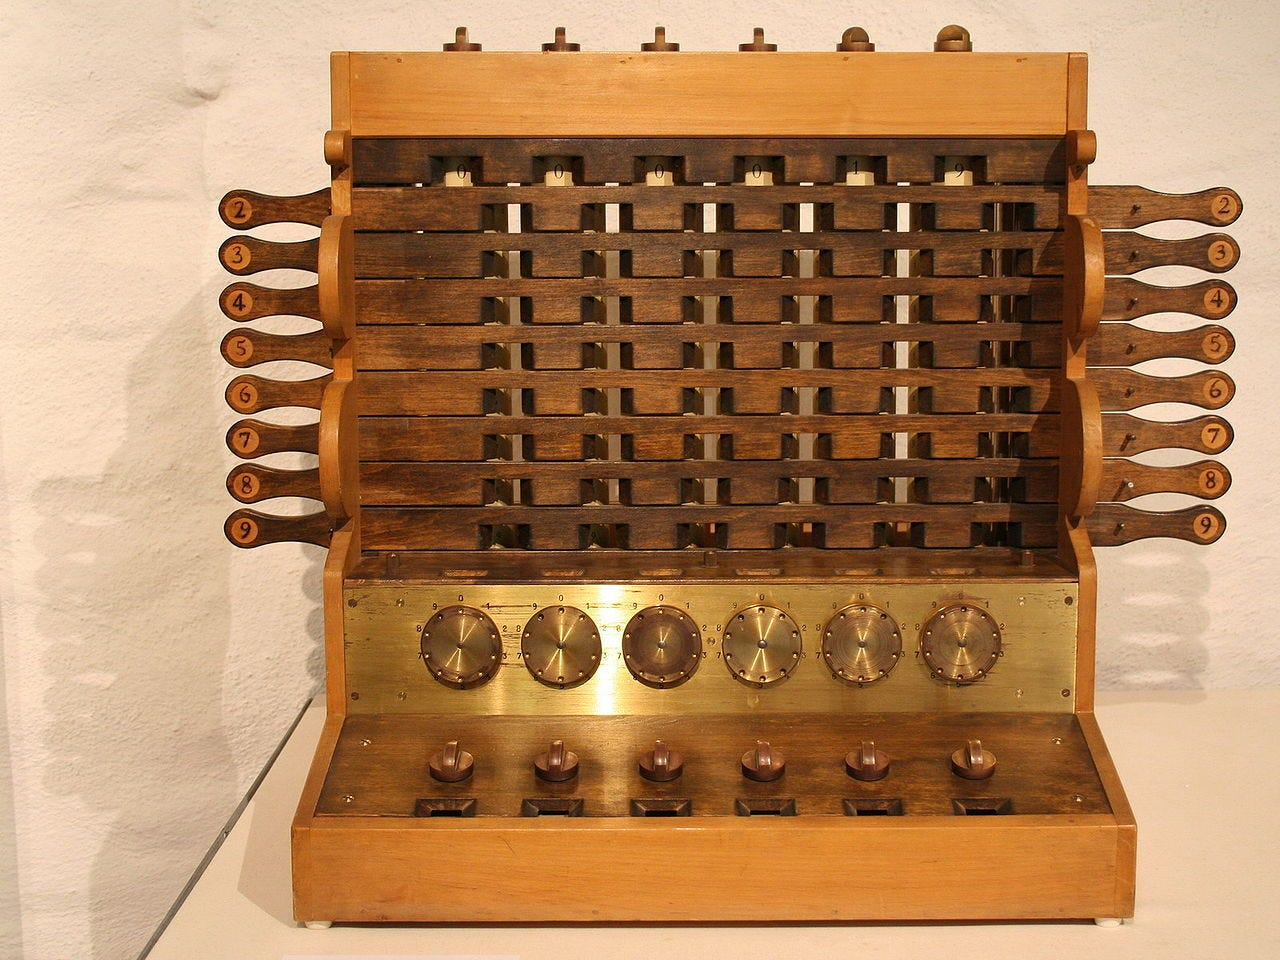
\includegraphics[width=0.9\textwidth]{schickard-machine}
  \url{https://www.youtube.com/watch?v=5undFLMNohA&t=2s}
\end{frame}

\begin{frame}{Ранни изчислителни устройства /сметачки/}
  1642 г. - Blaise Pascal’s ``Pascaline''
  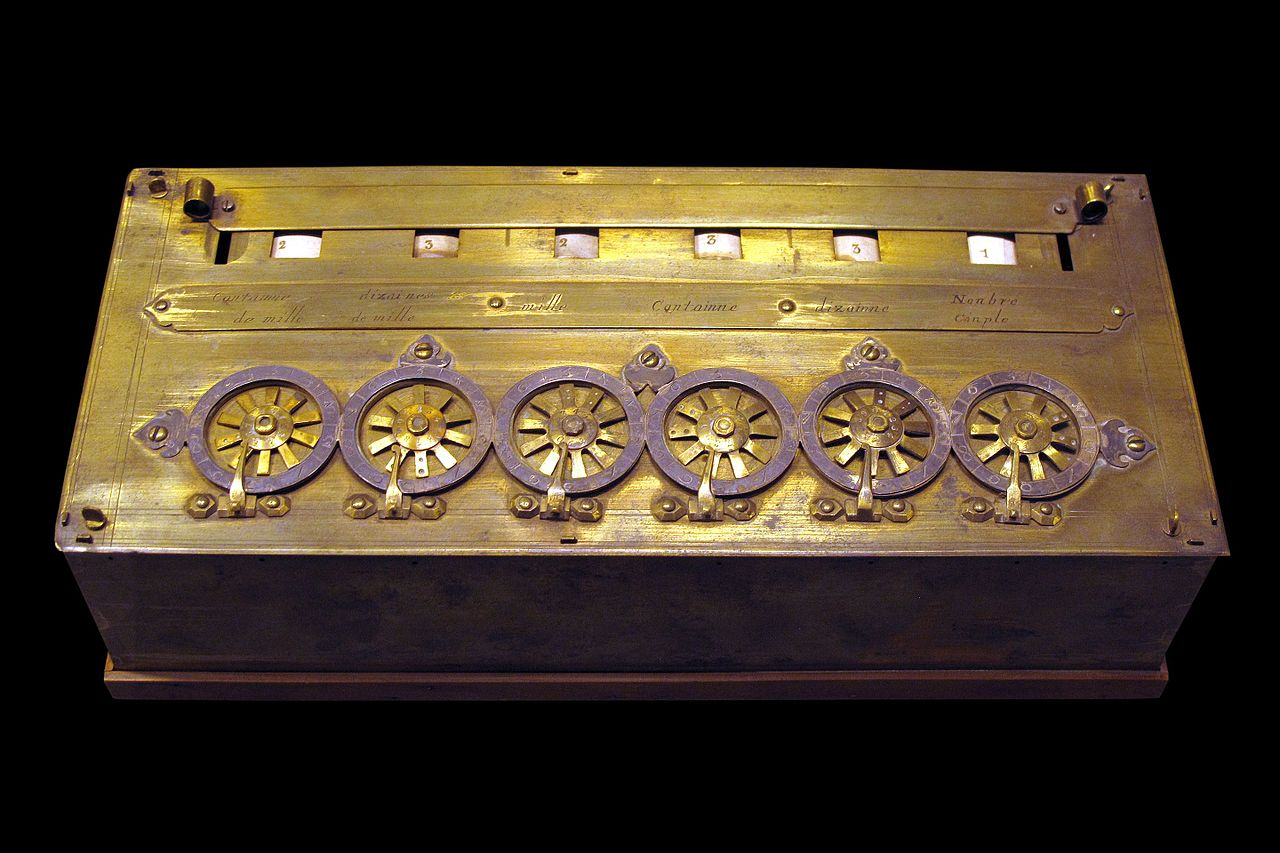
\includegraphics[width=0.9\textwidth]{pascaline}
  \url{https://www.youtube.com/watch?v=3h71HAJWnVU}
\end{frame}


\begin{frame}[plain]{Ранни изчислителни устройства /сметачки/}
  
  - 1834 Чарлз Бабидж

  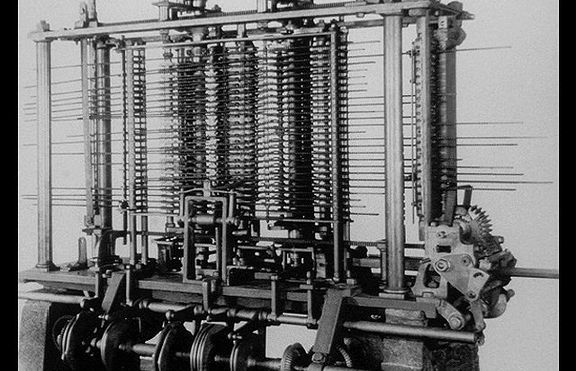
\includegraphics[width=\textwidth]{babidge}

\end{frame}


\begin{frame}[plain]{Ранни изчислителни устройства /сметачки/}
  
  - 1834 Чарлз Бабидж

\textit{``През 1834 година конструкторът \underline{замислил} създаването на механично устройство, способно не просто да сумира, но и да управлява хода на собствената си работа, в зависимости от заложена програма и резултатите от междинните изчисления! Последователността на изчисленията в машината на Бабидж се определяла от перфокарти с програма.''}

\end{frame}



\begin{frame}{1935 - 1945}

  - Konrad Zuse, Германия 

  - Alan Turing, Англия

  - Harold Keen, САЩ

  - Дж. Атанасов, САЩ

  - George Stibitz, САЩ

  \scriptsize по \url{https://www.youtube.com/watch?v=qundvme1Tik}
\end{frame}

\begin{frame}{Konrad Zuse}
  постига дизайн на компютър, които получава последователност от дупки върху перфокарти 
\end{frame}


\begin{frame}{Harold Keen}
  Машина за нелинейни диференциални уравнения
\end{frame}

\begin{frame}{Дж. Атанасов}
  Машина за алгебрични уравнения
\end{frame}


\begin{frame}[plain]{George Stibitz}
  Експериментира с набор от релета за съставяне на подходящи електр. вериги за реализиране на двоична логика

  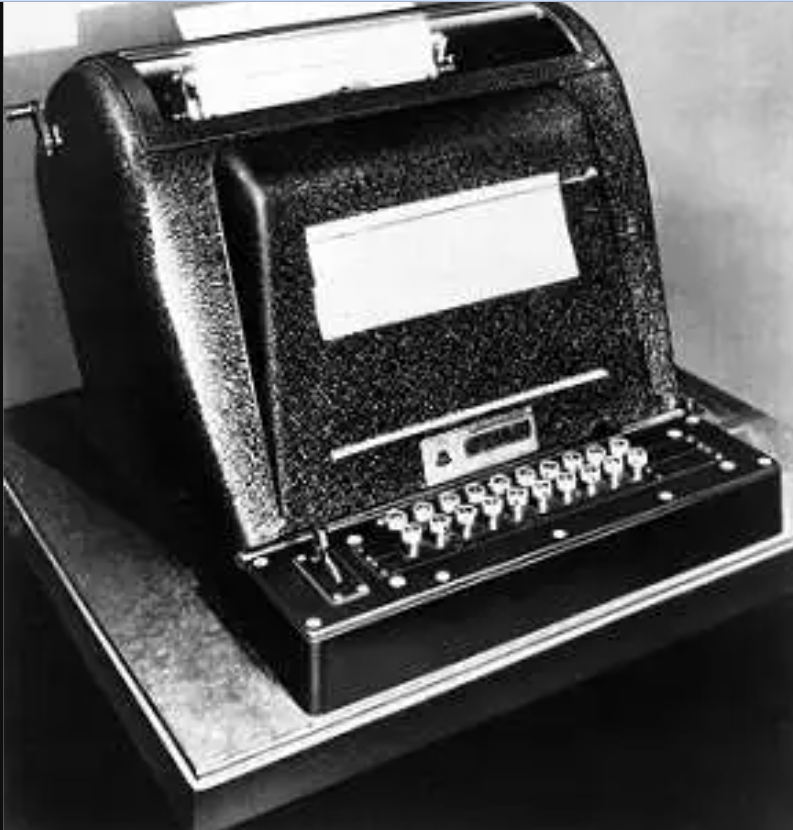
\includegraphics[width=0.5\textwidth]{stibitz-machine}

  \url{https://www.edn.com/stibitz-demonstrates-remote-computing-september-11-1940/}
\end{frame}




\begin{frame}[plain, fragile]{1946 - 1950}

  по \url{https://www.youtube.com/watch?v=wsirYCAocZk}

  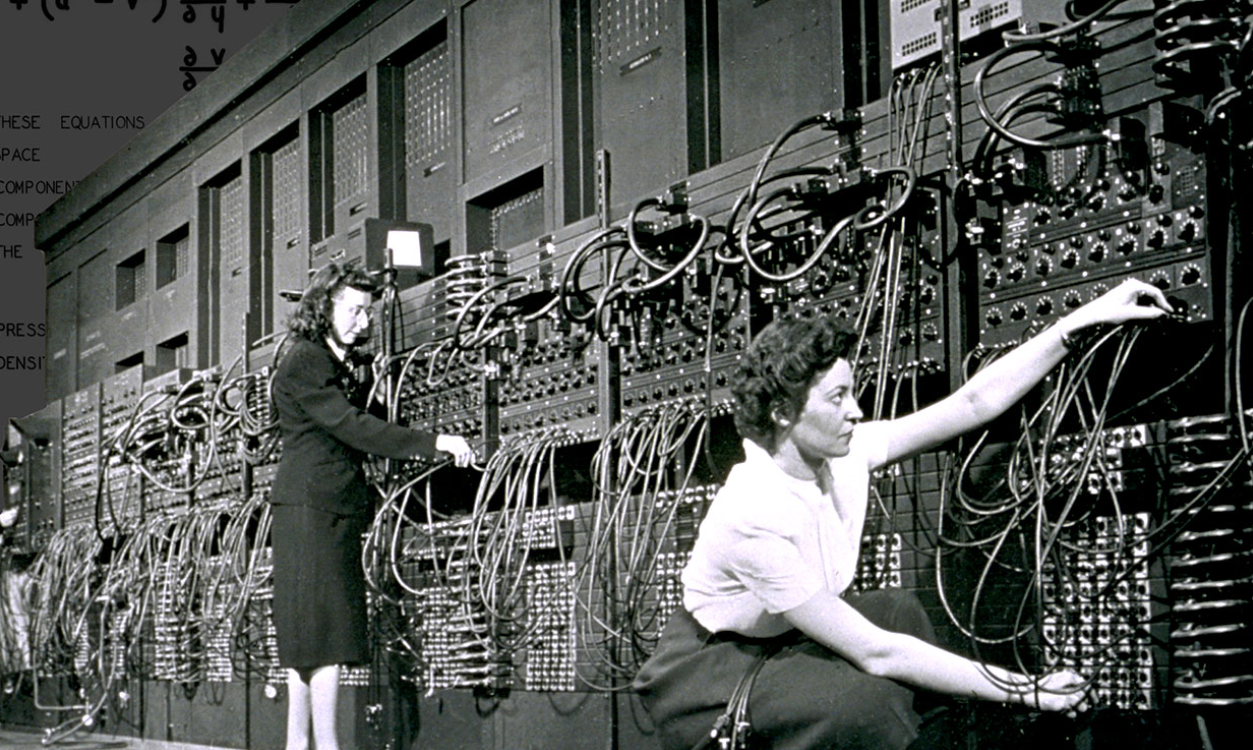
\includegraphics[width=0.9\textwidth]{eniac}

  ENIAC (Electronic Numerical Integrator and Computer)

  Presper Eckert and John Mauchly

  \url{https://www.kaldata.com/it-%D0%BD%D0%BE%D0%B2%D0%B8%D0%BD%D0%B8/%D0%BD%D0%B5%D1%80%D0%B0%D0%B7%D0%BA%D0%B0%D0%B7%D0%B0%D0%BD%D0%B0%D1%82%D0%B0-%D0%B8%D1%81%D1%82%D0%BE%D1%80%D0%B8%D1%8F-%D0%B7%D0%B0-%D0%BA%D0%BE%D0%BC%D0%BF%D1%8E%D1%82%D1%80%D0%B8%D1%82%D0%B5-311231.html}
\end{frame}


\begin{frame}[plain, fragile]{1946 - 1950}

  EDSAC (Cambridge), IAS (USA),  UNIVAC-1 (USA, първият компютър на пазара)

  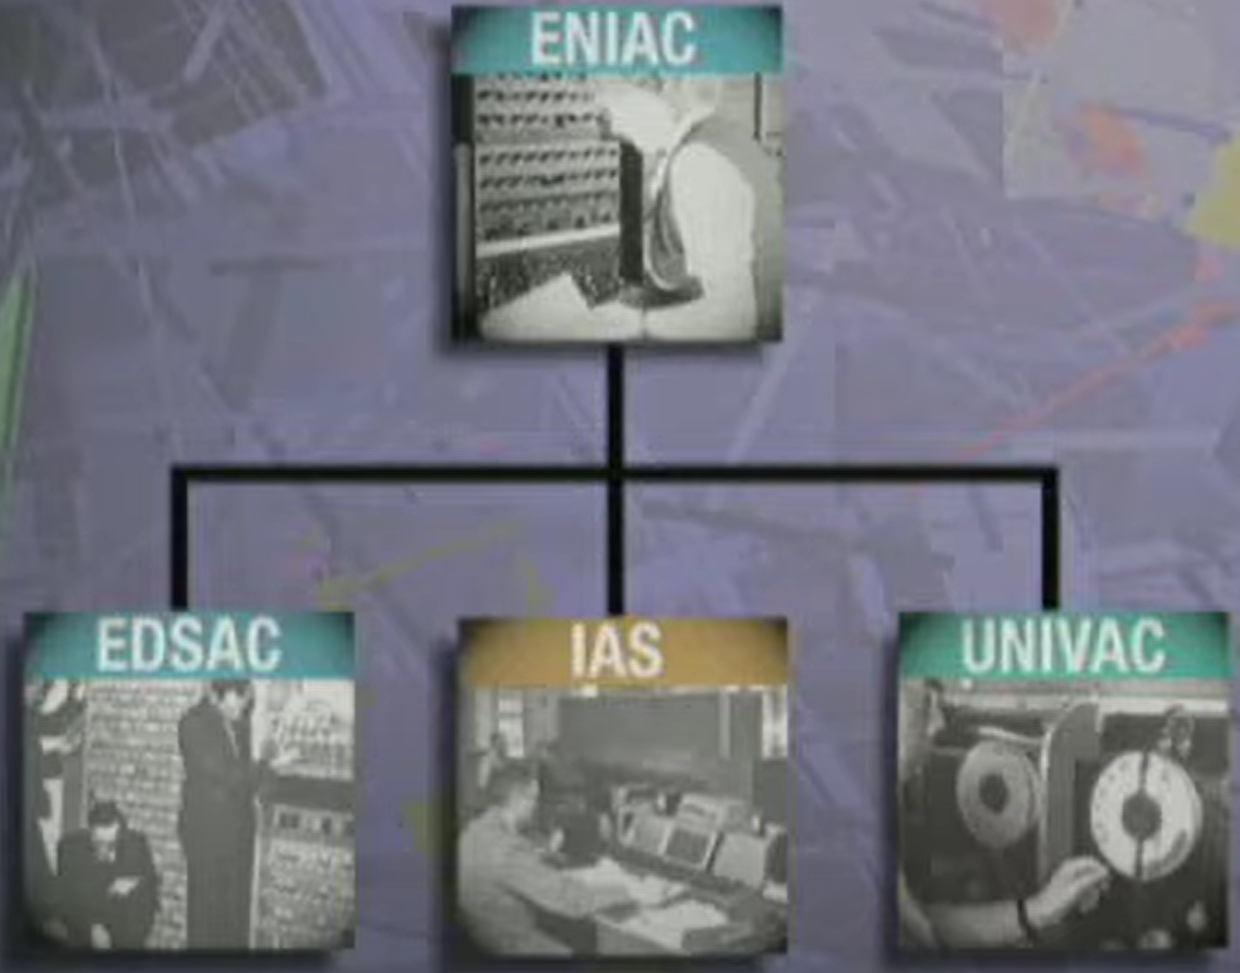
\includegraphics[width=0.7\textwidth]{eniac-desc}

\end{frame}


\begin{frame}[plain, fragile]{1946 - 1950}

  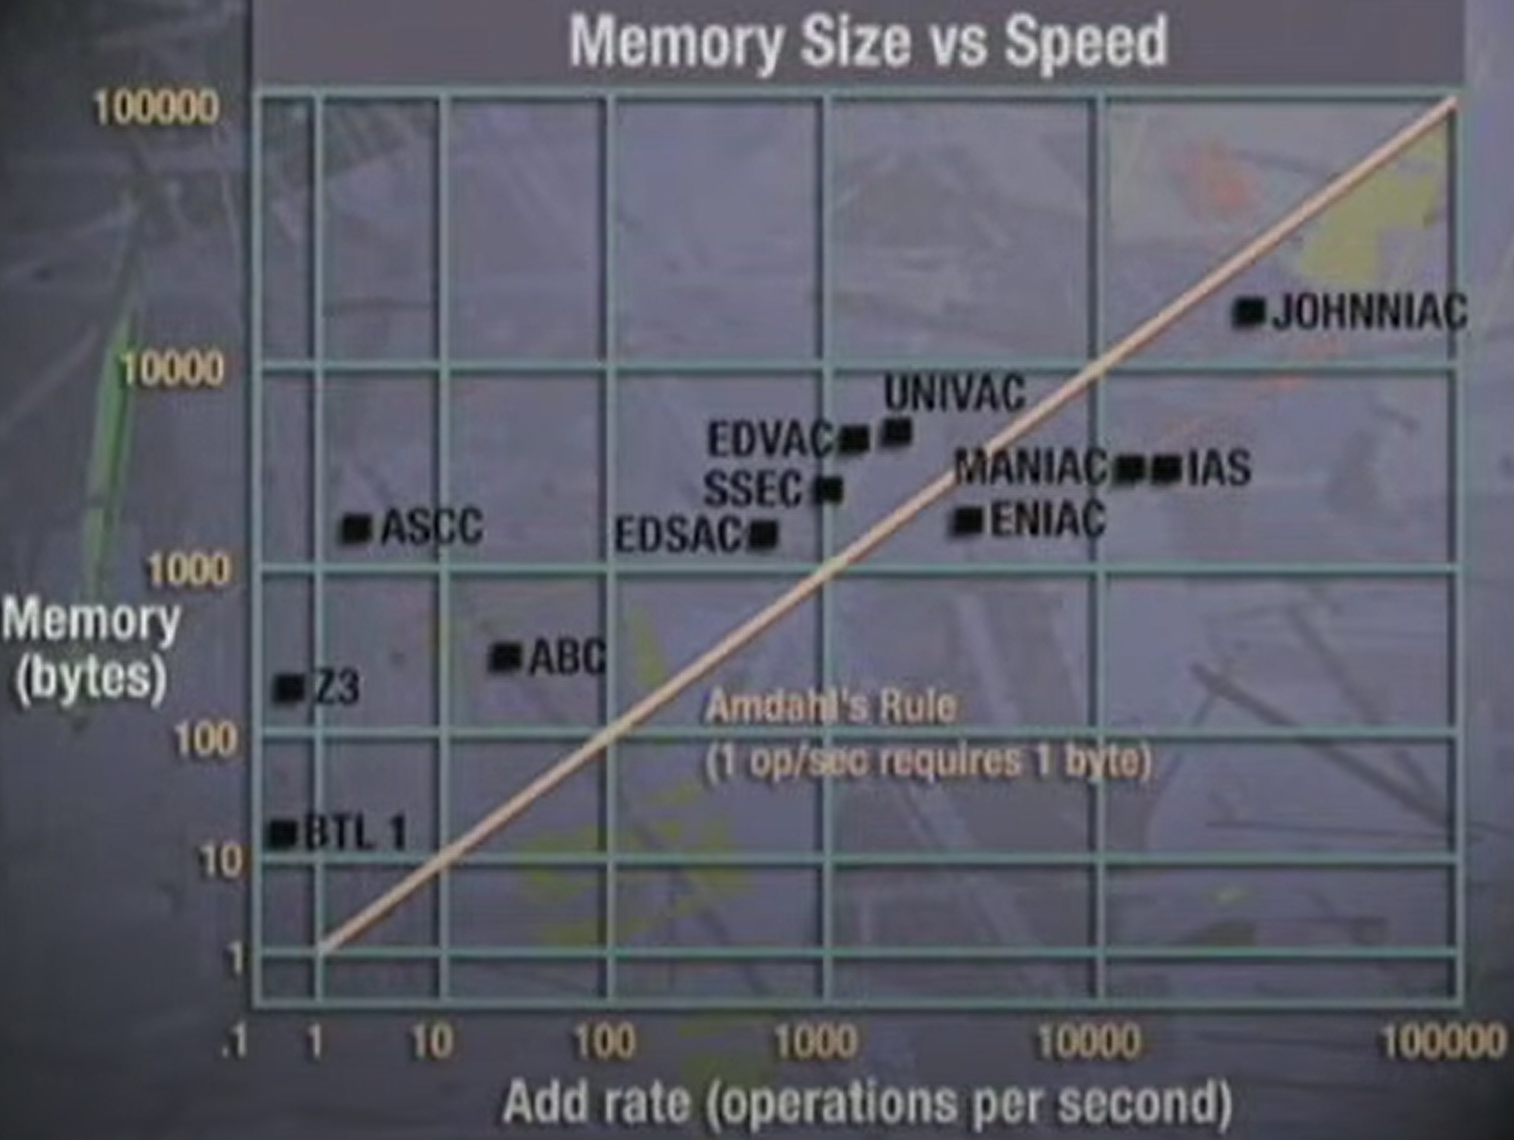
\includegraphics[width=0.85\textwidth]{memory-speed}

\end{frame}


\begin{frame}[plain, fragile]{1946 - 1950}

  EDVAC - бързо подаване на интрукции и памет

  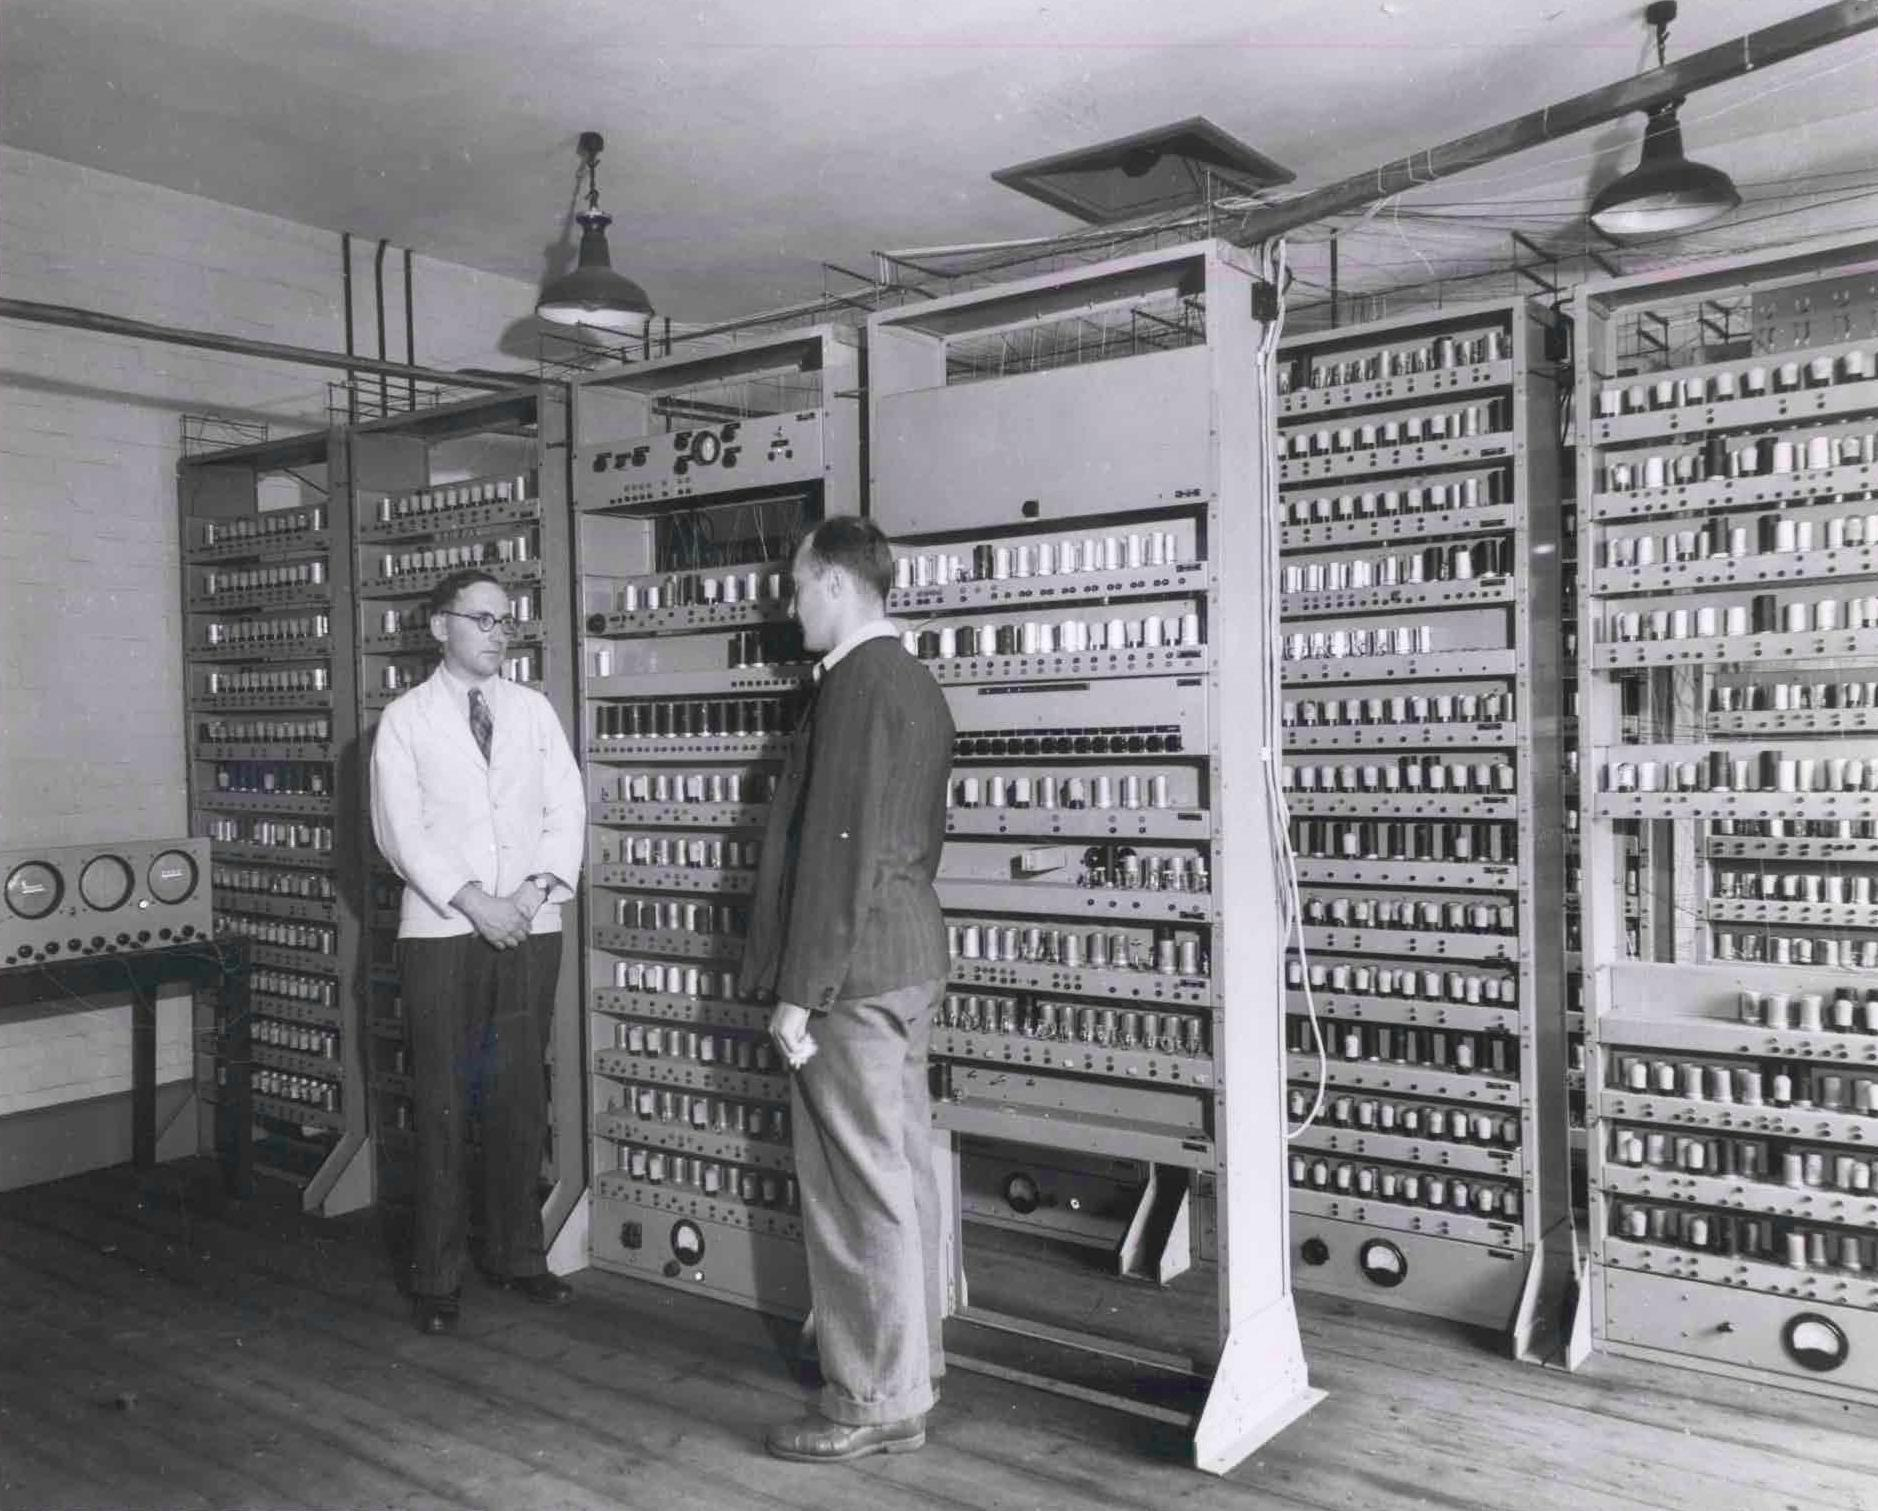
\includegraphics[width=\textwidth]{edvac}

\end{frame}

\begin{frame}[plain, fragile]{1946 - 1950}

  \url{https://web.mit.edu/STS.035/www/PDFs/edvac.pdf}

  \centering
  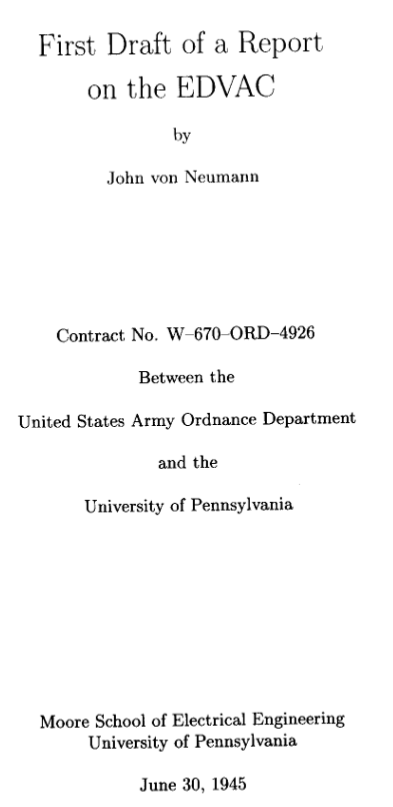
\includegraphics[width=0.33\textwidth]{first-draft-neumann}
\end{frame}




\begin{frame}[plain]{Суперкомпютри}

  \url{https://top500.org/lists/top500/2024/06/}
  \centering
  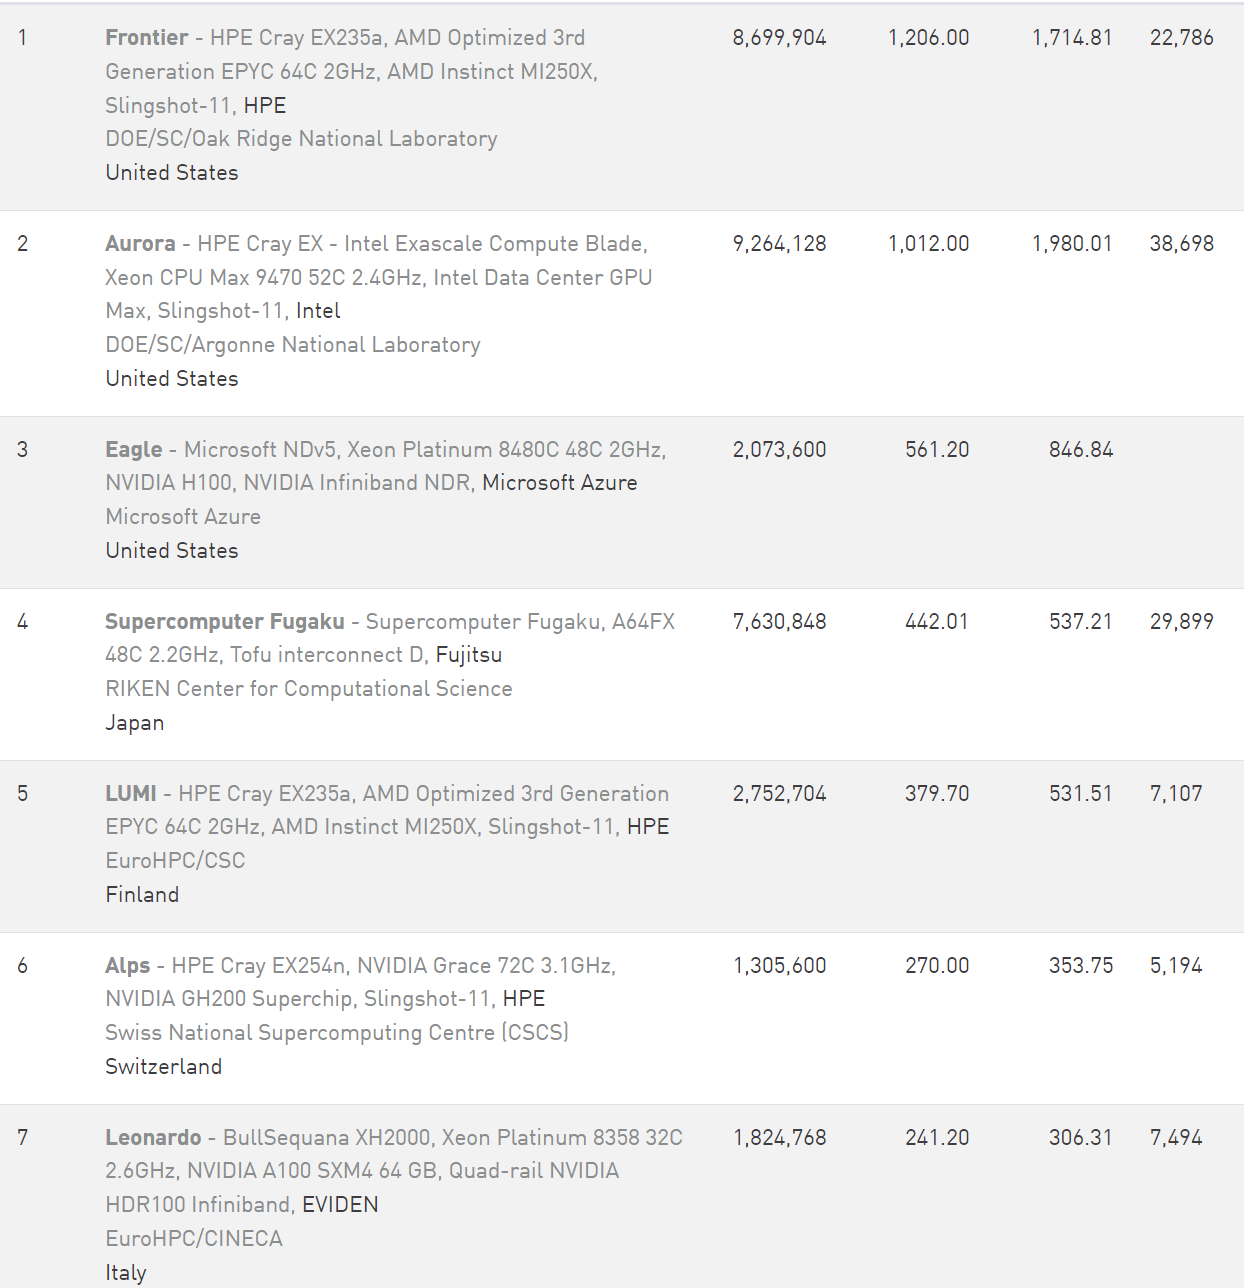
\includegraphics[width=0.7\textwidth]{top500-supercomp}
  
\end{frame}





\section{Основни C++ конструкции за паралелни изчисления.}

%%%%%%%%%%%%%%%%%%%%%%%%%%%%%%%%%%%%%
\begin{frame}[fragile]{Основни C++ конструкции.}
  Домашна работа:
  
  \url{https://github.com/EricDarve/cme213-spring-2021/tree/main/Lecture%20Slides/cpp%20tutorial}

  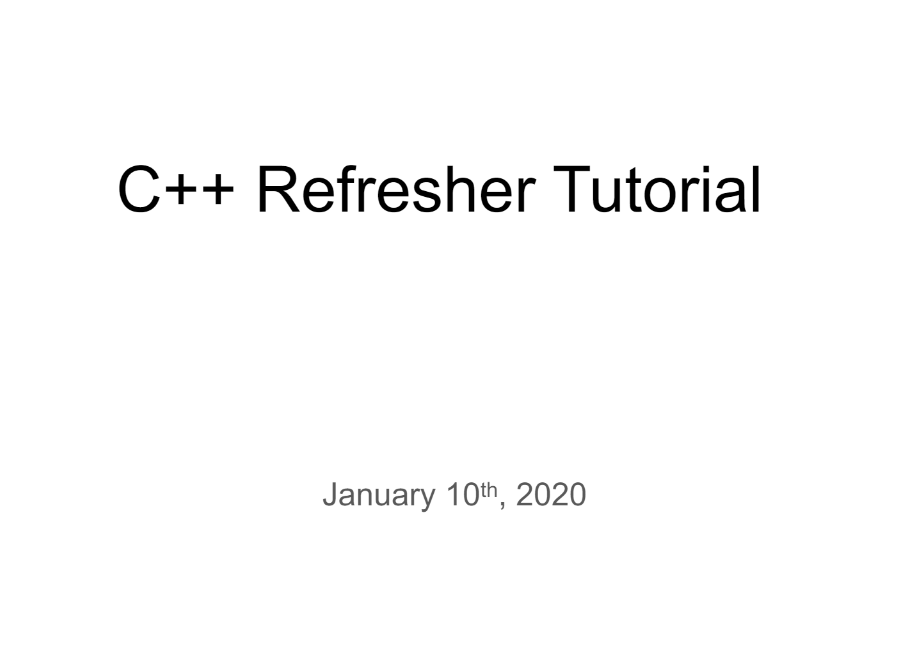
\includegraphics[width=\textwidth]{cpp-refresher}
\end{frame}

%%%%%%%%%%%%%%%%%%%%%%%%%%%%%%%%%%%%%

\begin{frame}[fragile]
  \frametitle{Достъп до отдалечен компютър}

\begin{verbatim}
ssh -X -p 65000 име@neutronstar.iaps.institute
\end{verbatim}

или


\centering
\includegraphics[width=0.3\textwidth]{putty}

  \url{https://www.putty.org/}
\end{frame}

\end{document}

%%% Local Variables:
%%% mode: latex
%%% TeX-master: t
%%% End:


